\subsection{Rayos x: Funciones de distribución de pares}

La función distribución radial (RDF) parcial describe la probabilidad de 
encontrar un átomo de tipo B en un cascarón a una distancia $r$ de un 
átomo de referncia de tipo A y está definida por la siguiente formula
\begin{equation}
    g_{AB}(r) = \frac{V}{4 \pi r^2 N_B} \sum_{i}^{N_A} \sum_{j\neq i}^{N_B} \delta(r - r_{ij}),
\end{equation}
donde $N_A$ y $N_B$ son los números de átomos de tipo A y B, respectivamente,
$V$ es el volumen de la celda de simulación y $r_{ij}$ es la distancia entre
los átomos $i$ y $j$. Estas curvas se calculan y presentan en la Figura 
\ref{fig:srdfs} para las distintas permutaciones de A y B (Li-Li, Si-Li, Si-Si).

\begin{figure}[h!]
    \centering
    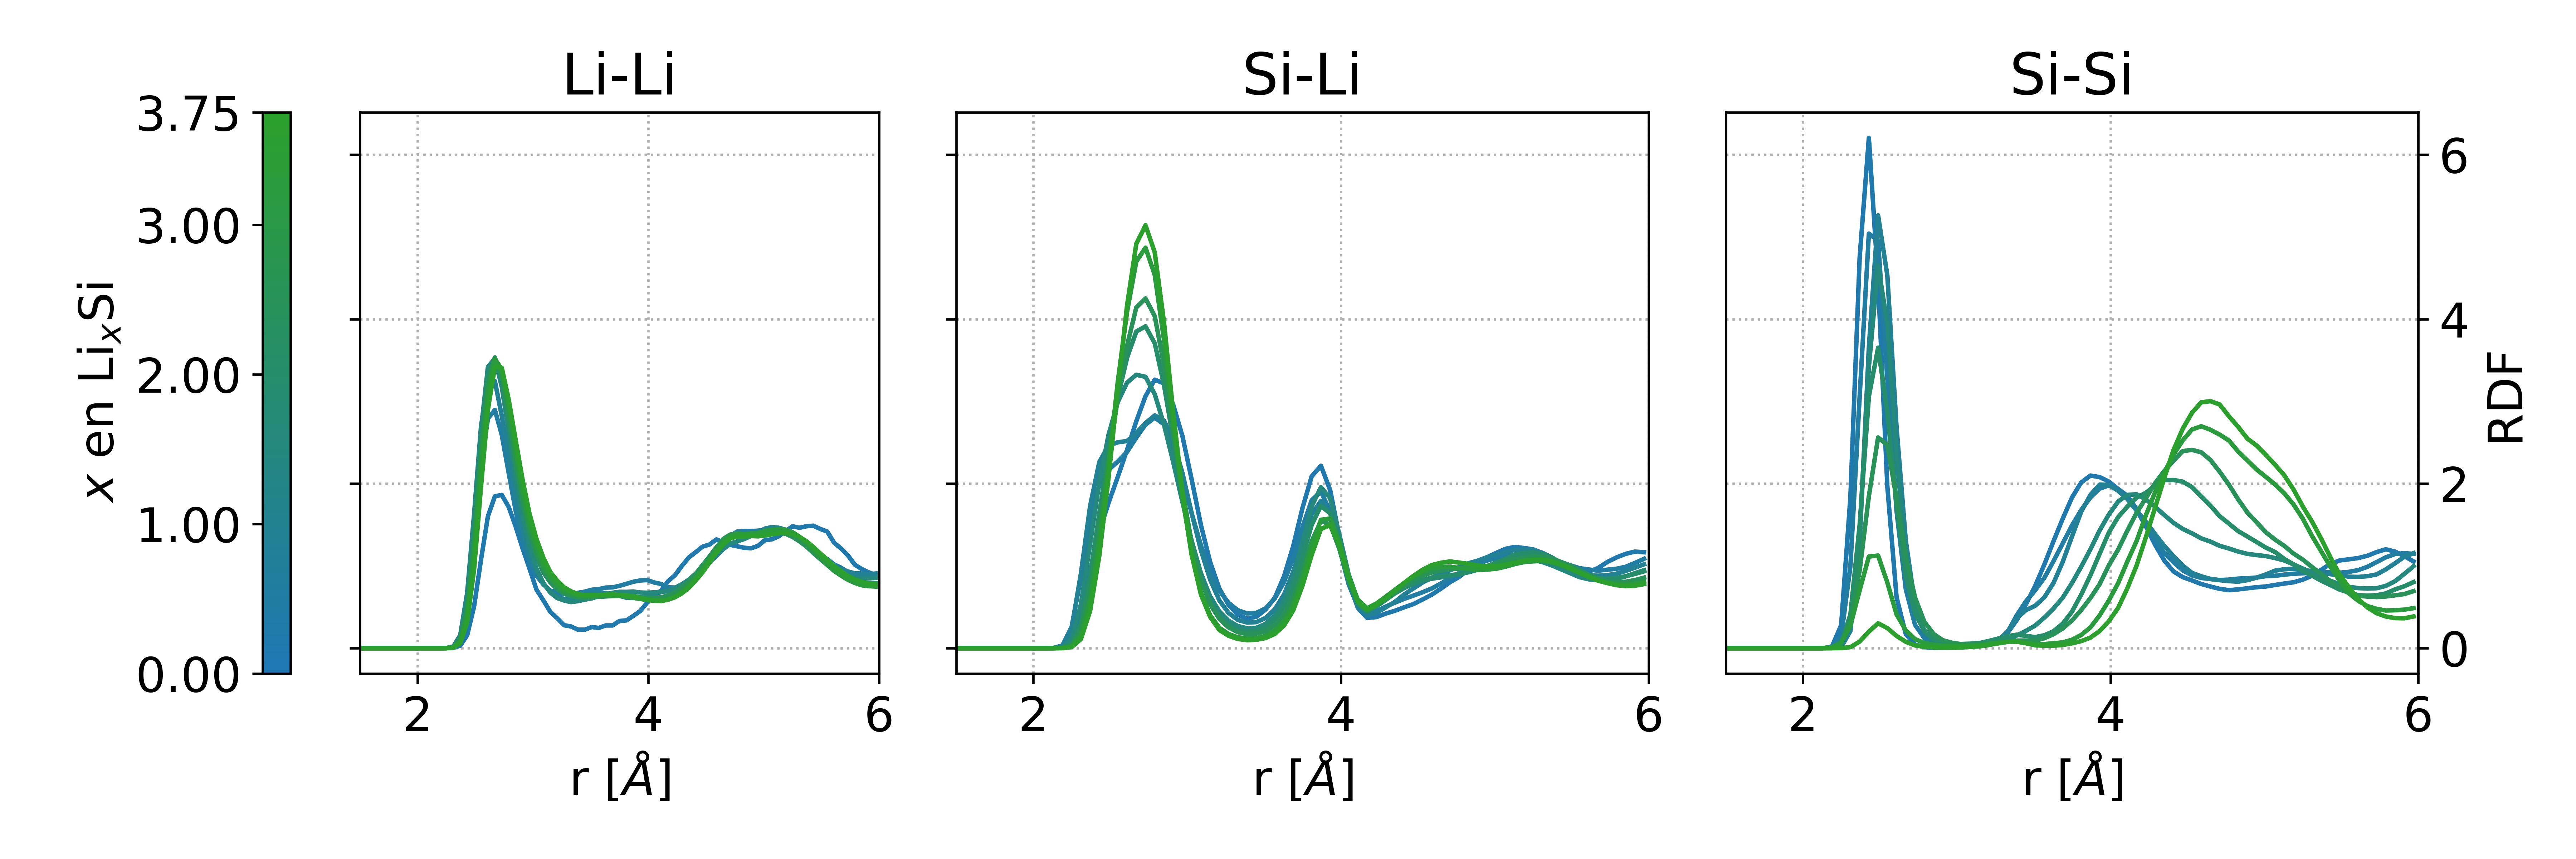
\includegraphics[width=\textwidth]{Silicio/prediccion/resultados/xray/prdfs.png}
    \caption{RDFs parciales para Li-Li, Si-Li y Si-Si para los valores $x$ en 
    Li$_x$Si optimizados. El color de la curva cambia de azul (predominio del Si)
    a verde (predominio del Li). Las barras de error son menores que el ancho de 
    las líneas.}
    \label{fig:prdfs}
\end{figure}

Luego, la función distribución radial de a pares $G(r)$ puede calularse utilizando
que \cite{billing2019}
\begin{equation}
    G(r) = 4 \pi r \rho_0 \left[\sum_{\langle A,B \rangle} \frac{b_A b_B}{\langle b\rangle^2} g_{AB}(r) - 1\right], 
\end{equation}
donde $\rho_0$ es la densidad de la celda de simulación, $\langle A, B \rangle$
considera las permutaciones sin repeticiones de A y B, $b_A$ y $b_B$ son los 
factores de dispersión de los átomos A y B, respectivamente, y $\langle b \rangle$
es el factor de dispersión promedio de la celda de simulación. Los factores de 
dispersión para Li y Si son 3 y 14, respectivamente, lo que resulta en una 
contribución del 82\% para la RDF parcial de Si-Si, un 16\% para la Si-Li y
un 3\% para la Li-Li.

Para el calculo de la $G(r)$ del Si litiado se consideraron contribuciones 
de cada estructura $s \in \lbrace$c-Si, c-Li$_{15}$Si$_4$, a-Si, 
a-Li$_{15}$Si$_4\rbrace$ presentes en el experimento con distintos pesos,
\begin{equation}\label{eq:contributions}
    G(r) = \sum_s w_s \cdot G_s(r),
\end{equation}
donde cada $G_s(r)$ se presenta en la Figura \ref{fig:gofrs}. Para el 
ajuste de los pesos de las estructuras se minimizó el error cuadrático 
medio y se obtuvieron los valores que se presentan en la Tabla 
\ref{t:w-gofrs}.

\begin{figure}[h!]
    \centering
    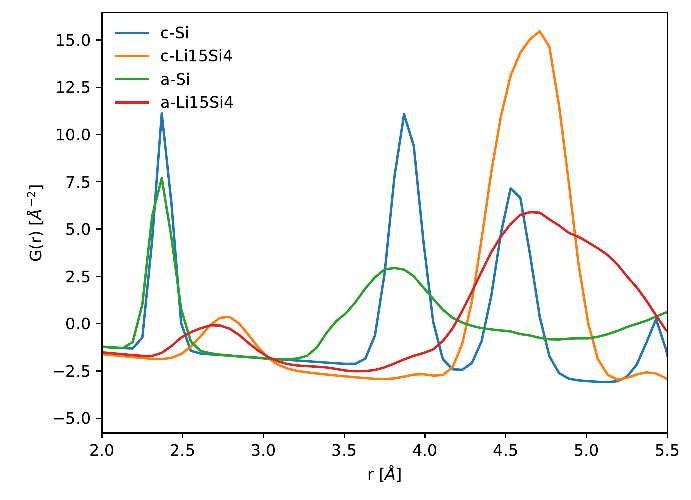
\includegraphics[width=.7\textwidth]{Silicio/prediccion/resultados/xray/gofrs.png}
    \caption{Funciones de distribución de pares $G(r)$ de estructuras 
    cristalinas y amorfas utilizadas para calcular las curvas de la Figura 
    \ref{fig:pdfs}.}
    \label{fig:gofrs}
\end{figure}

\begin{table}[h!]
    \centering
    \caption{Factor de peso de cada contribución (c-Si, c-Li$_{15}$Si$_4$, a-Si y 
    a-Li$_{15}$Si$_4$) a la función distribución radial de a pares $G(r)$ del 
    Si litiado (ver las Figuras \ref{fig:gofrs} y \ref{fig:pdfs} y la ecuación 
    \ref{eq:contributions}). El porcentaje de cada peso se agrega entre paréntesis.}
    \setlength\extrarowheight{2pt}\stackon{%
    \begin{tabular}{l c c c c}
        \toprule
        \textbf{Ajuste} & 
        \textbf{c-Si} & 
        \textbf{c-Li$_{15}$Si$_4$} & 
        \textbf{a-Si} & 
        \textbf{a-Li$_{15}$Si$_4$} \\ 
        \midrule
        cristalino & 0.03358 (30.15\%) & 0.077784 (69.85\%) & -- & -- \\
        DFTB amorfo & 0.0 (0.0\%) & 0.036422 (9.78\%) & 0.187971 (50.48\%) & 0.147955 (39.74\%) \\
        \bottomrule
    \end{tabular}
    }{}
    \label{t:w-gofrs}
\end{table}

\begin{figure}[h!]
    \centering
    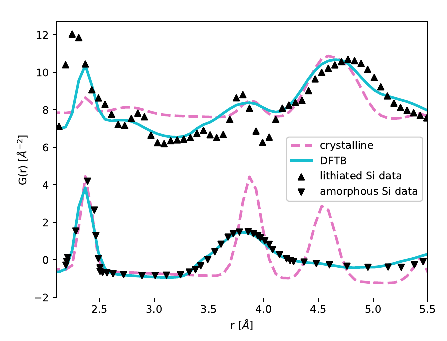
\includegraphics[width=.7\textwidth]{Silicio/prediccion/resultados/xray/pdfs.png}
    \caption{Funciones de distribución de pares $G(r)$ para Si amorfo y 
    completamente litiado contrastadas con datos experimentales. Los triángulos 
    que apuntan hacia abajo corresponden al experimento de a-Si de Laaziri 
    \textit{et al.} \cite{laaziri1999}, mientras que los que apuntan hacia arriba 
    corresponden al experimento de Key \textit{et al.} \cite{key2011}. Las curvas 
    DFTB azules consideran tanto las estructuras cristalinas y amorfas. Las 
    contribuciones de cada una están en la Tabla  \ref{t:w-gofrs}. Los datos del Si 
    litiado tienen una contribución extra de 8 \AA$^{-2}$ para tener las dos curvas 
    en el mismo gráfico. Las barras de error son menores que el ancho de las líneas.}
    \label{fig:pdfs}
\end{figure}
